\documentclass{article}

\usepackage{geometry}
\usepackage{amsmath}
\usepackage{graphicx, eso-pic}
\usepackage{listings}
\usepackage{hyperref}
\usepackage{multicol}
\usepackage{fancyhdr}
\pagestyle{fancy}
\fancyhf{}
\hypersetup{ colorlinks=true, linkcolor=black, filecolor=magenta, urlcolor=cyan}
\geometry{ a4paper, total={170mm,257mm}, top=40mm, right=20mm, bottom=20mm, left=20mm}
\setlength{\parindent}{0pt}
\setlength{\parskip}{0.5em}
\renewcommand{\headrulewidth}{0pt}
\AddToShipoutPictureBG{%
  \AtPageUpperLeft{%
    \raisebox{-\height}{
\includegraphics[width=\paperwidth, height=30mm]{../headerarkav.png}}
  }
}
\rfoot{\thepage}
\lfoot{Competitive Programming - Arkavidia 8.0}
\lstset{
    basicstyle=\ttfamily\small,
    columns=fixed,
    extendedchars=true,
    breaklines=true,
    tabsize=2,
    prebreak=\raisebox{0ex}[0ex][0ex]{\ensuremath{\hookleftarrow}},
    frame=none,
    showtabs=false,
    showspaces=false,
    showstringspaces=false,
    prebreak={},
    keywordstyle=\color[rgb]{0.627,0.126,0.941},
    commentstyle=\color[rgb]{0.133,0.545,0.133},
    stringstyle=\color[rgb]{01,0,0},
    captionpos=t,
    escapeinside={(\%}{\%)}
}
\begin{document}

\begin{center}
    \section*{D. Desa Arkavidia} % ganti judul soal

    \begin{tabular}{ | c c | }
        \hline
        Batas Waktu  & 1s \\    % jangan lupa ganti time limit
        Batas Memori & 256MB \\  % jangan lupa ganti memory limit
        \hline
    \end{tabular}
\end{center}

\subsection*{Deskripsi}
Pada kota Arkavidia, terdapat $N$ desa bernomor $1$ sampai $N$. Terdapat $N-1$ jalan yang masing-masing jalan menghubungkan dua desa berbeda. Tidak ada dua jalan yang menghubungkan dua desa yang sama. Setiap desa dapat pergi ke desa lain dengan menggunakan jalan yang tersedia.

Akhir-akhir ini, terdapat pencuri yang sering mencuri desa-desa di kota Arkavidia. Untungnya, walikota Arkavidia dapat menyewa penjaga untuk menangani kasus pencurian. Walikota dapat meminta penjaga untuk berjaga di desa $i$ dan penjaga tersebut akan menjaga desa $i$ dan desa-desa yang dihubungkan langsung dengan desa $i$ melalui satu jalan saja.

Tentukan banyak penjaga minimal yang harus disewa walikota agar semua desa di kota Arkavidia terjaga dari pencuri.

\subsection*{Format Masukan}
Baris pertama terdiri dari sebuah bilangan bulat $N$  ($1 \leq$ $N$ $\leq$ $2 \times 10^5$), menyatakan banyaknya desa di kota Arkavidia.

$N-1$ baris berikutnya terdiri dari dua buah bilangan $U$ dan $V$ ($1 \leq$ $U$, $V$ $ \leq$ $N$; $U$ $\neq$ $V$) yang menyatakan terdapat jalan yang menghubungkan desa $U$ dan desa $V$ secara langsung.

\subsection*{Format Keluaran}
Tuliskan banyaknya penjaga minimal yang dibutuhkan.

\begin{multicols}{2}
\subsection*{Contoh Masukan 1}
\begin{lstlisting}
7
1 2
3 4
2 3
3 5
5 6
4 7
\end{lstlisting}
\columnbreak

\subsection*{Contoh Keluaran 1}
\begin{lstlisting}
3
\end{lstlisting}
\vfill
\null
\end{multicols}

\begin{multicols}{2}
\subsection*{Contoh Masukan 2}
\begin{lstlisting}
8
1 2
1 3
1 4
1 5
1 6
6 7
7 8
\end{lstlisting}
\columnbreak

\subsection*{Contoh Keluaran 2}
\begin{lstlisting}
2
\end{lstlisting}
\vfill
\null
\end{multicols}

\pagebreak
\subsection*{Penjelasan}
Pada testcase pertama, susunan desa pada kota Arkavidia adalah sebagai berikut:

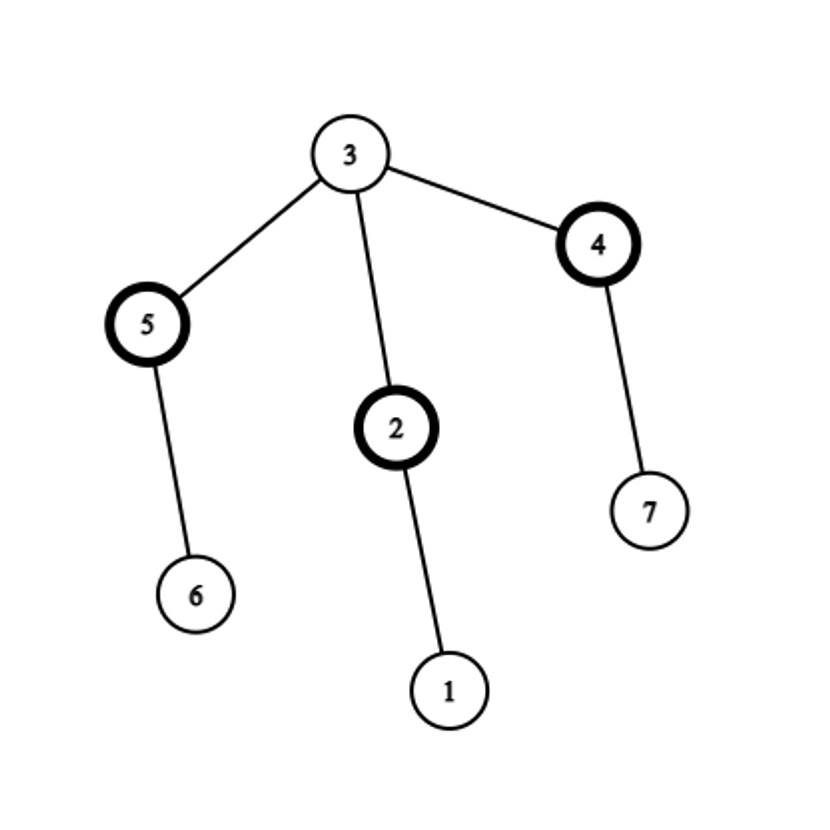
\includegraphics[width=225px]{graph.png}

Walikota dapat menyimpan 3 penjaga pada desa 2, 4, dan 5.

\end{document}